% AKULIN--KARLOV Fig.20.4, R2 CP09: original-based 2D projection of Lorenz attractor.
% Geometry traced editorially from the 626x630 printed scan, NOT a numerical
% solution of Lorenz ODEs. Preserve the two funnels, route labels 1/2/3, A/B,
% transverse planes, guide dashes and visibly decreasing coils in funnel 2.
\documentclass[border=5pt]{standalone}
\usepackage{fontspec,unicode-math}
\setmainfont{Noto Serif}
\setmathfont{STIXTwoMath-Regular.otf}
\usepackage{tikz}
\usetikzlibrary{arrows.meta,calc}
\tikzset{
 axis/.style={draw=black,line width=.82pt,-{Latex[length=2.3mm,width=1.3mm]}},
 plane/.style={draw=black,line width=.76pt},
 traj/.style={draw=black,line width=1.02pt,line cap=round,line join=round},
 boldtraj/.style={draw=black,line width=1.33pt,line cap=round,line join=round},
 hidden/.style={draw=black,line width=.84pt,dash pattern=on 4pt off 3.2pt},
 label/.style={font=\fontsize{12}{14}\selectfont,inner sep=1pt},
 pathlabel/.style={font=\fontsize{16}{18}\selectfont\itshape,inner sep=1pt}}
\begin{document}
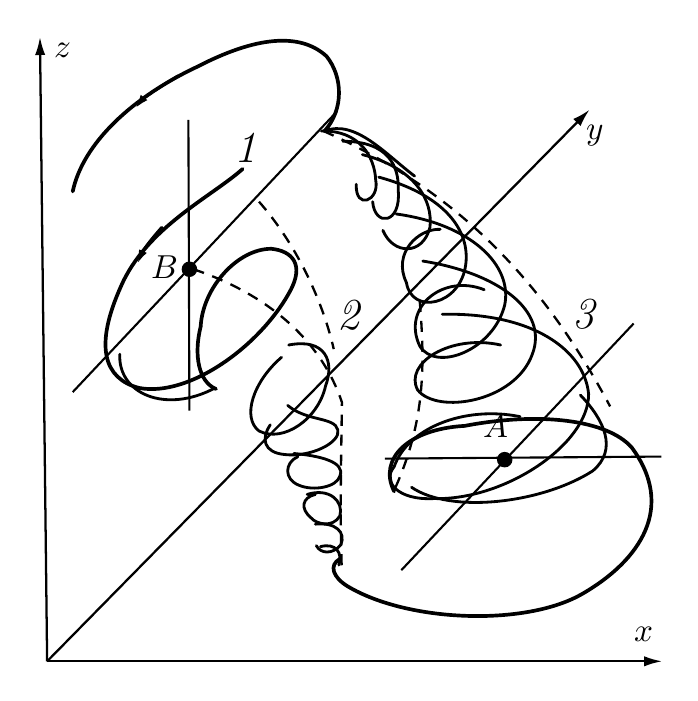
\begin{tikzpicture}[x=.013cm,y=-.013cm]
\path[use as bounding box] (0,0) rectangle (627,630);
% Author's three projected axes. Upper right diagonal is y, not a cone edge.
\draw[axis] (19,619)--(620,619); \node[label,anchor=east] at (615,593) {$x$};
\draw[axis] (19,619)--(549,80); \node[label,anchor=west] at (543,105) {$y$};
\draw[axis] (19,619)--(12,9); \node[label,anchor=west] at (23,22) {$z$};
% Physical affine cutting lines through B and A (as in 1987 original).
\draw[plane] (44,356)--(302,82);
\draw[plane] (157,90)--(158,374);
\draw[plane] (365,530)--(592,289);
\draw[plane] (349,421)--(619,419);
% Initial incoming trajectory 1: exceptionally wide overhead bend, return to B.
\draw[boldtraj] (44,160) .. controls (54,113) and (102,68) .. (166,38)
 .. controls (222,9) and (266,4) .. (292,28)
 .. controls (308,48) and (309,80) .. (290,101);
\draw[traj,-{Latex[length=1.8mm,width=1.1mm]}] (147,47) .. controls (127,59) and (113,69) .. (105,79);
\draw[traj] (290,101)..controls (320,89) and (350,124)..(378,145);
% B-side wide winding. Distinct loops are visible as increasingly narrow ellipses.
\draw[boldtraj] (210,138)..controls (180,165) and (116,195)..(91,253)
 ..controls (65,311) and (74,343)..(109,352)
 ..controls (158,361) and (227,311)..(256,258)
 ..controls (271,231) and (258,218)..(238,216)
 ..controls (205,216) and (171,254)..(169,292)
 ..controls (162,320) and (167,346)..(184,353);
\draw[traj] (90,319)..controls (88,357) and (134,378)..(183,352);
\draw[traj,-{Latex[length=1.8mm,width=1.1mm]}] (131,195)..controls (123,204) and (114,215)..(107,231);
% B is intersection of oblique plane cut and z-parallel B line.
\fill (158,236) circle (2.8pt); \node[label,anchor=east] at (149,234) {$B$};
\draw[hidden] (162,236) .. controls (239,262) and (288,309)..(307,366)
 .. controls (306,436) and (305,478)..(307,533);
% Funnel 2 begins as a wide loop and contracts toward the vertical foot.
\draw[traj] (255,310)..controls(291,303) and (300,326)..(291,350)
 ..controls(284,382) and (250,406)..(226,394)
 ..controls(209,381) and (220,346)..(248,322);
\draw[traj] (254,369)..controls (273,385) and (300,380)..(303,393)
 ..controls (306,405) and (277,420)..(251,417)
 ..controls (230,415) and (228,401)..(237,388);
\draw[traj] (260,416)..controls (284,418) and (311,424)..(305,438)
 ..controls (302,449) and (279,453)..(265,447)
 ..controls (250,441) and (251,425)..(264,419);
\draw[traj] (273,456)..controls (295,449) and (309,463)..(305,477)
 ..controls (298,489) and (282,485)..(277,479)
 ..controls (266,470) and (268,459)..(281,456);
\draw[traj] (281,485)..controls (301,483) and (311,493)..(306,505)
 ..controls (298,515) and (286,514)..(282,506);
\draw[traj] (286,507)..controls(301,503) and (308,513)..(304,525);
% Left cone envelope; dashed guide is an auxiliary boundary, never a trajectory.
\draw[hidden] (226,170)..controls (262,211) and (288,266)..(299,314);
\node[pathlabel] at (313,281) {2};
% Passage over upper arc: broadened, overlapping turns on right (funnel 3).
% These loops are open in 2D projection and NOT false additional intersections.
\draw[traj] (287,101)..controls (324,100) and (339,126)..(340,149)
 ..controls (344,169) and (320,179)..(321,153);
\draw[traj] (308,111)..controls (353,111) and (363,136)..(362,159)
 ..controls (365,192) and (339,195)..(337,170);
\draw[traj] (327,124)..controls (378,137) and (396,168)..(393,195)
 ..controls (386,223) and (357,222)..(347,198);
\draw[traj] (343,146)..controls (409,164) and (432,199)..(428,231)
 ..controls (423,272) and (375,281)..(370,249)
 ..controls (356,220) and (382,196)..(403,197);
\draw[traj] (360,182)..controls (433,192) and (474,232)..(466,271)
 ..controls (455,315) and (399,337)..(383,311)
 ..controls (365,273) and (406,240)..(446,256);
\draw[traj] (386,228)..controls (461,240) and (509,277)..(493,319)
 ..controls (476,366) and (400,378)..(381,354)
 ..controls (367,328) and (413,299)..(462,310);
\draw[traj] (405,280)..controls (493,278) and (544,315)..(548,358)
 ..controls (548,407) and (466,462)..(397,460)
 ..controls (361,462) and (346,443)..(358,429)
 ..controls (371,391) and (427,369)..(481,380);
\draw[hidden] (289,101)..controls (426,162) and (507,254)..(569,370);
\draw[hidden] (383,267)..controls (388,328) and (389,384)..(358,452);
\node[pathlabel] at (543,280) {3};
% A-side broad lower loop, almost planar xy, and return to other wing.
\draw[boldtraj] (358,453) .. controls (342,421) and (372,392)..(427,389)
 .. controls (500,375) and (566,383)..(590,410)
 .. controls (633,468) and (599,520)..(542,553)
 .. controls (487,585) and (372,581)..(313,546)
 .. controls (298,537) and (294,525)..(305,519);
\draw[traj] (375,449)..controls (413,475) and (502,465)..(552,433)
 ..controls(577,412) and (563,383)..(540,359);
% A lies at intersection of A's horizontal and oblique guide.
\fill (466,422) circle (2.8pt); \node[label,anchor=south west] at (442,404) {$A$};
% Author arrow on the initial B trajectory, not a new state or a vertex.
\node[pathlabel] at (213,117) {1};
\end{tikzpicture}
\end{document}
